\chapter{System Evaluation}
This chapter discusses the different types of tests that were carried out throughout the project’s lifecycle to ensure that all features of the project worked as intended and resulted in a project which the client would be satisfied using in their business on a daily basis. 

\section{Testing Overview}
Testing played a large part in the development cycle due to the nature of the project. This ensured that bugs were found and disposed of early in development.\\
Some testing methodologies used were: 
\begin{itemize}
    \item Unit Testing
    \item Functional Testing
    \item Integration Testing
    \item Usability Testing
    \item Security Testing
    \item Compatibility Testing
    \item Acceptance  Testing
\end{itemize}
\newpage

\section{Unit Testing}
Unit testing was carried out on each layer of the system. This ensured that each component in the system carried out their functionality correctly. Unit testing was carried out both manually and automatically throughout.

\subsection{Web Application Unit Testing}
The web application components were tested manually after being built, as well as automatically tested using a testing software called selenium after a section of the project was completed. This was done by creating test cases which were created and run after the development of each section. These were then all run frequently to ensure that correct functionality of components was occurring.

\subsection{Server Unit Testing}
Unit tests were carried out on the server side ensuring all calculations are valid. This was a vital aspect as these values must be sent to the government, so correct testing was very important. PyTest was used to achieve this process. Also all parts of the API server were tested using Postman to ensure that everything was working as intended.  All tests pass and code coverage for all calculations that are coverable via usage of just unit tests is one hundred percent.
\begin{figure}[h!]
 	\caption{Sample of Server Unit Tests}
	\label{image:unittests}
 	\centering
 	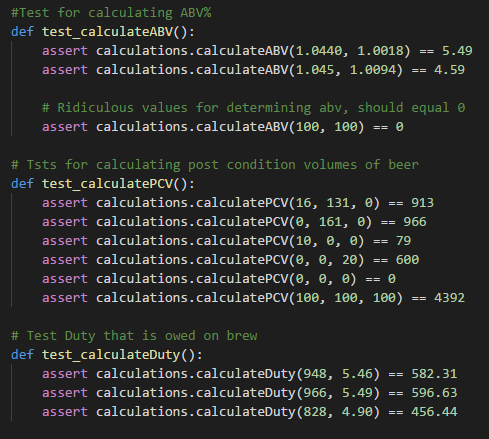
\includegraphics[width=0.9\textwidth]{Images/unittesting.PNG}
\end{figure}
\newpage

\section{Functional Testing}
Functional testing was carried out automatically on the server side to ensure that the database was being populated correctly with data that would be sent to the server. Then the calculations carried out on the data were correct and then delete them from the database. This was all carried out using a test database and using PyTest as the method of testing calculations. Functional testing was also carried out manually on all parts of the web application to ensure functionality.  All tests pass and code coverage for all calculations that are coverable via usage of just functional tests is one hundred percent. This results in one hundred percent code coverage of the calculations file methods between these functional tests and unit testing.
\begin{figure}[h!]
 	\caption{Sample of Server Functional Tests results}
	\label{image:unittests}
 	\centering
 	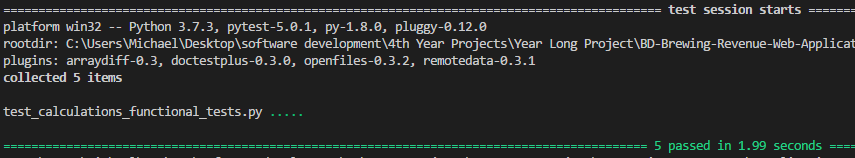
\includegraphics[width=1\textwidth]{Images/pytest results.PNG}
\end{figure}

\section{Usability Testing}
During weekly discussions with the project manager or client useability tests were carried out. New features of the project were displayed live and tested in front of meeting members. If they felt a change in a feature was necessary, then this was added as an issue to resolve in the next development cycle. 

\section{Integration Testing}
Integration testing was carried out every time a new component was added to the system. This was done to ensure that the newly installed component hadn’t caused issues in features of a previously working component and that the system as a whole was unaffected.

\section{Security Testing}
Security was carried out to ensure that all data was protected from unauthorized users. Testing was carried out to ensure these principles were covered with each security test.
\begin{itemize}
    \item Integrity
    \item Confidentiality
    \item Authentication
    \item Authorization
    \item Availability
    \item Non-repudiation
\end{itemize}
Tests were carried out on the web application ensuring non authorized members would not access pages. Tests were then also carried out on the API using Postman to ensure that if no authorization token was given data could not be accessed. 
\begin{figure}[h!]
 	\caption{Example of how Postman can test authorization with tokens}
	\label{image:autherror}
 	\centering
 	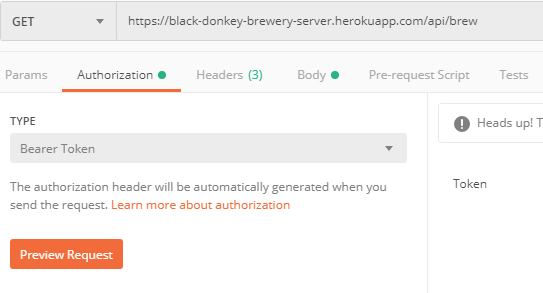
\includegraphics[width=0.9\textwidth]{Images/TokenTest.PNG}
\end{figure}
\newpage

\section{Compatibility Testing}
The application was tested in different environments to ensure functionality. The system was tested on different operating systems, browsers etc. This helps ensure that the application works for all users in different environments. The system was tested on four different browsers, Mozilla Firefox, Google Chrome, Microsoft Edge and Safari. It was also tested on Windows 7 and 10, Linux and macOS.
\begin{figure}[h!]
 	\caption{Test of application on different browsers simultaneously (Firefox and Google Chrome)}
	\label{image:browsertest}
 	\centering
 	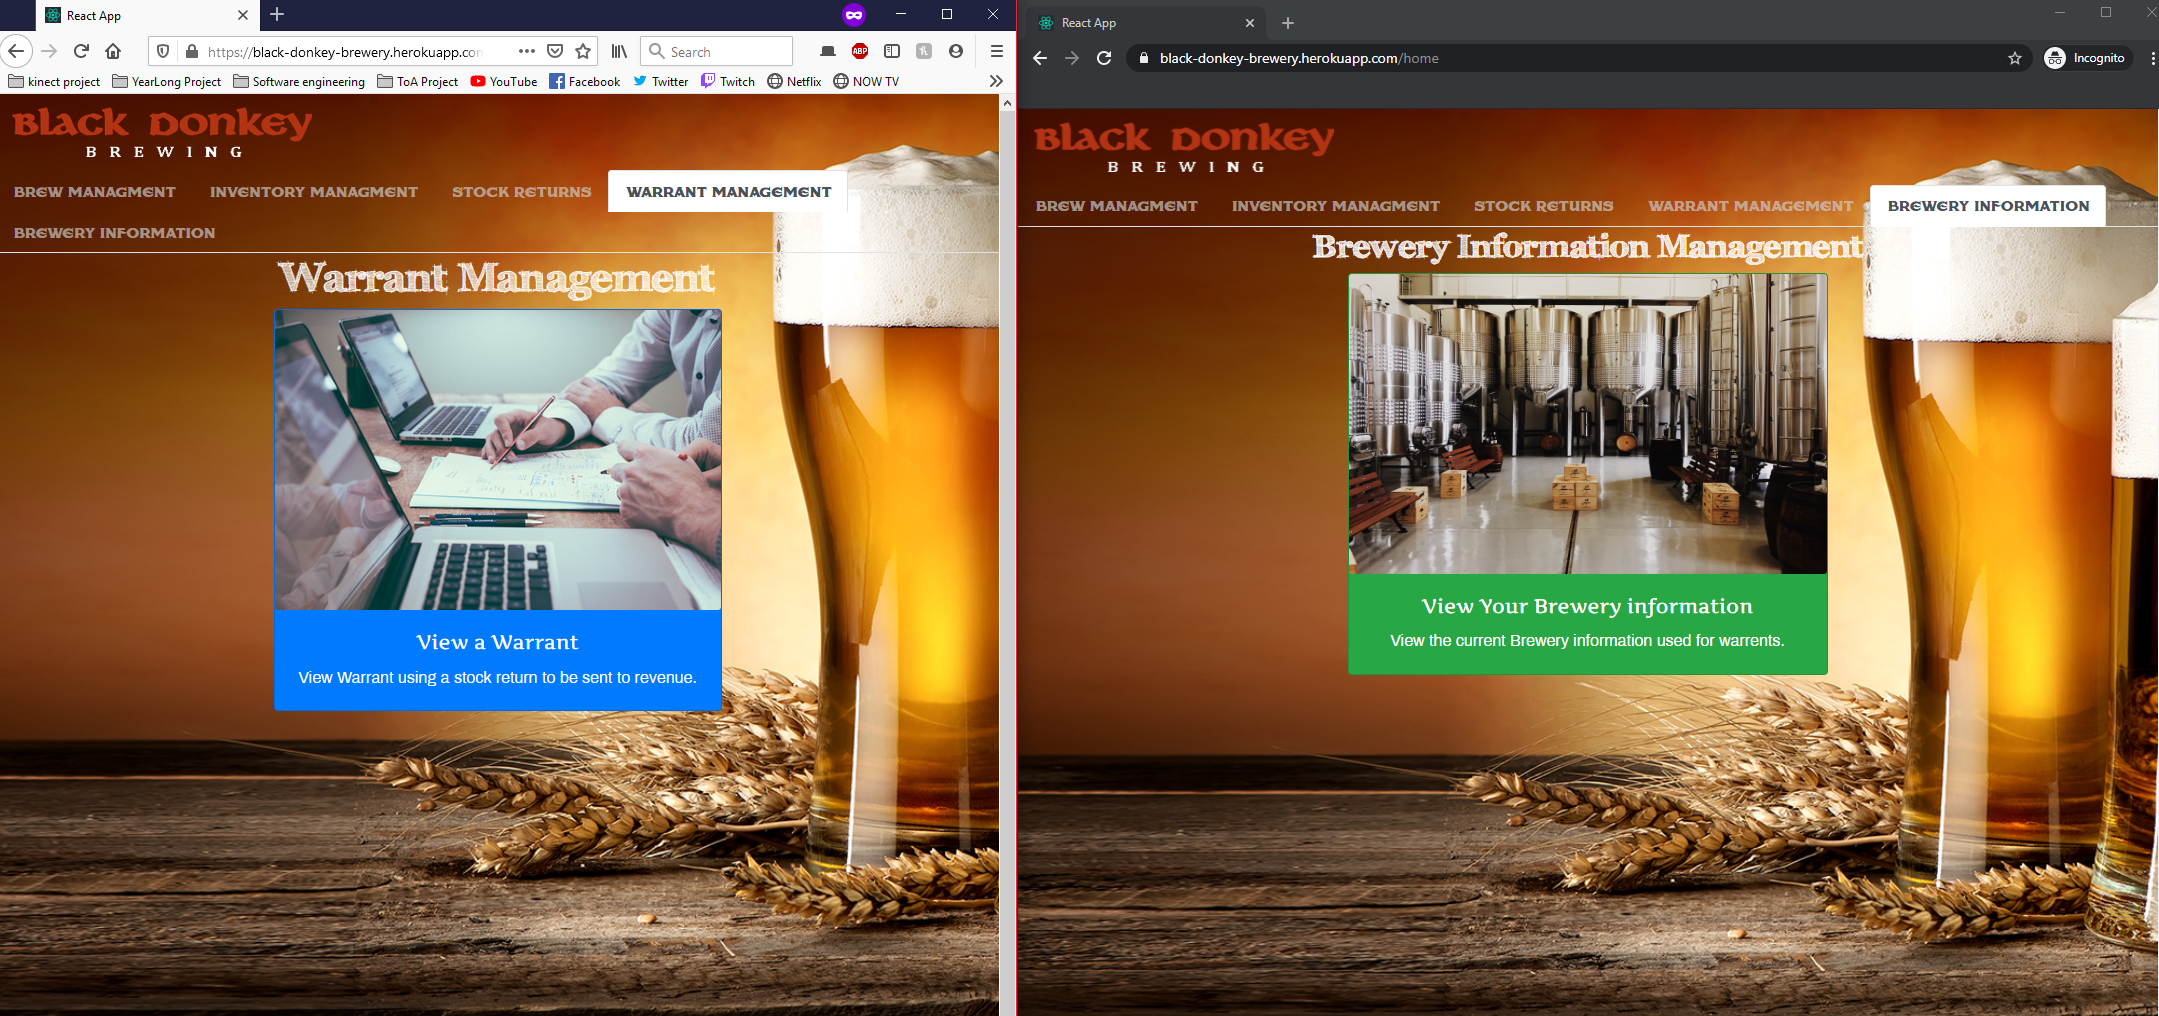
\includegraphics[width=1.0\textwidth]{Images/browser test.PNG}
\end{figure}
\newpage

\section{Performance Testing}
Load Testing was carried out using API Fortress, this was only tested when the application was placed on the cloud as API Fortress is a paid service, It was tested using a free trial only. This tested the website in a number of areas to see how it was able to perform. This testing ensured that a large amount of requests could be made to the API Server and handled at once without any issues. Load tests were limited on the free tier of Heroku as they only allowed a certain amount of requests to be made per hour. However the server coped perfectly well when tested using 100 requests per second for 30 seconds. This could be increased in a paid version of Heroku to try to get the maximum requests possible. The performance testing also looked at areas such as response times of the website in different areas of the world, some examples were 12ms response from London and 71ms response from Eastern United States.

\section{Acceptance Testing}
This was done to ensure that the product is ready for delivery. The project was handed over to the client to ensure it was of a proper standard and in a condition the client deemed to be acceptable as a final product. This led to feedback which would result in any changes to be made.

\newpage
\section{Limitations of Technology used}
Due to selecting such a versatile and adaptable selection of technologies limitations were not really an issue throughout development of the web application and server. Limitations started to creep into the project when deploying of the project to the cloud began to occur.  This was a result of selecting a free tier of cloud hosting. Heroku offers a free tier cloud hosting to users for their applications but as a result they offer less dynos (which Heroku uses to speed up your server) to free tier projects. To reduce costs of the project on the client this was a necessary sacrifice. This results in the user having to wait for a period of anywhere between ten seconds to a minute for the servers to start. Also the API server hosted on a separate Heroku server may not be up in time resulting in displaying no data to the user until it is online. This is an issue which could be addressed by moving to a paid tier of Heroku or use paid another cloud hosting service.